% Figure from MATH 591 notes, section 61 (Lecture 21).
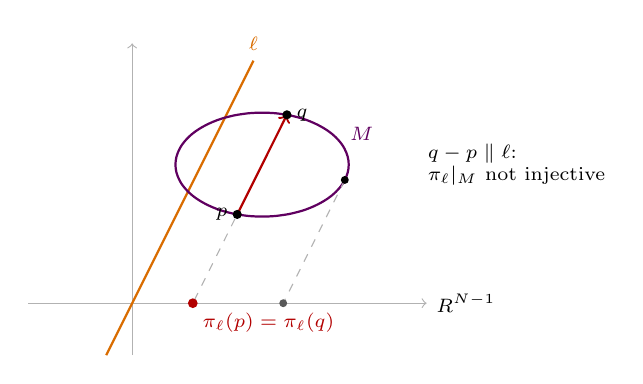
\begin{tikzpicture}[scale=1.1]
\draw[->, gray!60] (-1.2,0) -- (3.4,0) node[right, font=\scriptsize, text=black] {$\mathbb{R}^{N-1}$};
\draw[->, gray!60] (0,-0.6) -- (0,3.0);
\draw[orange!85!black, thick] (-0.3,-0.6) -- (1.4,2.8) node[above, font=\scriptsize] {$\ell$};
\draw[violet!75!black, thick] plot[smooth cycle] coordinates {(2.500,1.600) (2.497,1.647) (2.488,1.694) (2.472,1.740) (2.451,1.785) (2.424,1.830) (2.391,1.872) (2.353,1.913) (2.309,1.953) (2.260,1.990) (2.207,2.024) (2.149,2.056) (2.088,2.085) (2.022,2.112) (1.954,2.135) (1.883,2.154) (1.809,2.171) (1.733,2.183) (1.656,2.193) (1.578,2.198) (1.500,2.200) (1.422,2.198) (1.344,2.193) (1.267,2.183) (1.191,2.171) (1.117,2.154) (1.046,2.135) (0.978,2.112) (0.912,2.085) (0.851,2.056) (0.793,2.024) (0.740,1.990) (0.691,1.953) (0.647,1.913) (0.609,1.872) (0.576,1.830) (0.549,1.785) (0.528,1.740) (0.512,1.694) (0.503,1.647) (0.500,1.600) (0.503,1.553) (0.512,1.506) (0.528,1.460) (0.549,1.415) (0.576,1.370) (0.609,1.328) (0.647,1.287) (0.691,1.247) (0.740,1.210) (0.793,1.176) (0.851,1.144) (0.912,1.115) (0.978,1.088) (1.046,1.065) (1.117,1.046) (1.191,1.029) (1.267,1.017) (1.344,1.007) (1.422,1.002) (1.500,1.000) (1.578,1.002) (1.656,1.007) (1.733,1.017) (1.809,1.029) (1.883,1.046) (1.954,1.065) (2.022,1.088) (2.088,1.115) (2.149,1.144) (2.207,1.176) (2.260,1.210) (2.309,1.247) (2.353,1.287) (2.391,1.328) (2.424,1.370) (2.451,1.415) (2.472,1.460) (2.488,1.506) (2.497,1.553) (2.500,1.600)};
\node[violet!75!black, font=\scriptsize] at (2.650,1.950) {$M$};
\draw[gray!60, dashed] (1.787,2.175) -- (0.700,0);
\draw[->, thick, red!70!black] (1.213,1.025) -- (1.787,2.175);
\fill (1.213,1.025) circle (1.5pt) node[left, font=\scriptsize] {$p$};
\fill (1.787,2.175) circle (1.5pt) node[right, font=\scriptsize] {$q$};
\fill[red!70!black] (0.700,0) circle (1.6pt) node[below right, font=\scriptsize] {$\pi_\ell(p) = \pi_\ell(q)$};
\draw[gray!60, dashed] (2.455,1.423) -- (1.744,0);
\fill (2.455,1.423) circle (1.3pt); \fill[gray!70!black] (1.744,0) circle (1.3pt);
\node[font=\scriptsize, align=left, anchor=west] at (3.3,1.6) {$q - p \parallel \ell$:\\ $\pi_\ell|_M$ not injective};
\end{tikzpicture}
